\documentclass{article}
\usepackage{mathtools}
\usepackage{array}
\usepackage{graphicx}

\newcommand*{\addheight}[2][.5ex]{%
  \raisebox{0pt}[\dimexpr\height+(#1)\relax]{#2}%
}

% \documentclass[11pt,a4paper]{report}
\usepackage{tcolorbox}
\tcbuselibrary{minted,breakable,xparse,skins}

\definecolor{bg}{gray}{0.95}
\DeclareTCBListing{mintedbox}{O{}m!O{}}{%
  breakable=true,
  listing engine=minted,
  listing only,
  minted language=#2,
  minted style=default,
  minted options={%
    linenos,
    gobble=0,
    breaklines=true,
    breakafter=,,
    fontsize=\small,
    numbersep=8pt,
    #1},
  boxsep=0pt,
  left skip=0pt,
  right skip=0pt,
  left=25pt,
  right=0pt,
  top=3pt,
  bottom=3pt,
  arc=5pt,
  leftrule=0pt,
  rightrule=0pt,
  bottomrule=2pt,
  toprule=2pt,
  colback=bg,
  colframe=orange!70,
  enhanced,
  overlay={%
    \begin{tcbclipinterior}
    \fill[orange!20!white] (frame.south west) rectangle ([xshift=20pt]frame.north west);
    \end{tcbclipinterior}},
  #3}


\newcolumntype{R}[1]{>{\hbox to #1\bgroup\hfill$}c<{$\egroup}}
% Language setting
% Replace `english' with e.g. `spanish' to change the document language
\usepackage[english]{babel}

% Set page size and margins
% Replace `letterpaper' with `a4paper' for UK/EU standard size
\usepackage[letterpaper,top=2cm,bottom=2cm,left=3cm,right=3cm,marginparwidth=1.75cm]{geometry}

% Useful packages
\usepackage{amsmath}
\usepackage{graphicx}
\usepackage[colorlinks=true, allcolors=blue]{hyperref}
\usepackage{array}
\usepackage{setspace}   %Allows double spacing with the \doublespacing command

\newcolumntype{R}[1]{>{\hbox to #1\bgroup\hfill$}c<{$\egroup}}


\title{
  Exploration of the Hill Cipher\\
  \large Applied Methods in Linear Alg MTH-3130-001}
\author{By Rose Ordway, Sean Berna, and
Abby Castillo
}

% Title page



% Document body
\begin{document}
\renewcommand\arraystretch{1.2}
\doublespacing
\maketitle
\section*{Abstract}
Throughout this project, we examined the history of the Hill Cipher, including its past, present, and future applications, as well as its practicality in terms of computer security in modern times. Along with our research, we provide a mathematical foundation that demonstrates how each phase of the encryption can be deciphered with a basic understanding of linear algebra. This math involves multiplying matrices, inverting matrices, and computing a matrix's determinant. Throughout the course of the project, it became evident that the Hill Cipher is now obsolete, but it remains a famous example of linear algebra in encrypting. 

\section*{History of the Hill Cipher}
	\noindent Lester S. Hill was an American mathematician born in January of 1891 and lived until January of 1961; After receiving his first degree from Columbia College he received his Ph. D. from Yale University he continued his research and taught at the University of Montana, Princeton University, the University of Maine, Yale University and Hunter College (“Learn about Lester S. Hill”). One of Lester's most popular contributions to the field of mathematics is the research he did about the indirect correlation between an alphabet directly translated to numerical digits and its contents multiplied by a key matrix and its inverse. His paper about this can be found in volume 36 of The American Mathematical Monthly in an article Written by Lester Hill called “Cryptography in an Algebraic Alphabet” (Hill, 306). With this method in addition to translating a scrambled alphabet translation to digits, the user will need to figure out the size and contents of the key matrix used to encode and decode the encryption. 
 \\
 \\
In addition to the creation of the Hill Cipher, he also created a machine to encode and decode messages using this method. The name of the machine was named the message projector, this machine was patented in 1929 by Lester and his colleague, Louis Weisner, a mathematician who graduated from Columbia College with a Ph. D. in 1923 ( “Louis Weisner”). The purpose of the machine was described, as “to provide an improved machine for converting a message into a cipher message and for re-converting the cipher message into the original form of message.” (“US1845947A - Message Protector”).  Included below are diagrams of the message project found on the online documentation of the patent for the machine.

\noindent
\begin{center}

\begin{tabular}{|c|c|c|c|}
      \hline
      \addheight{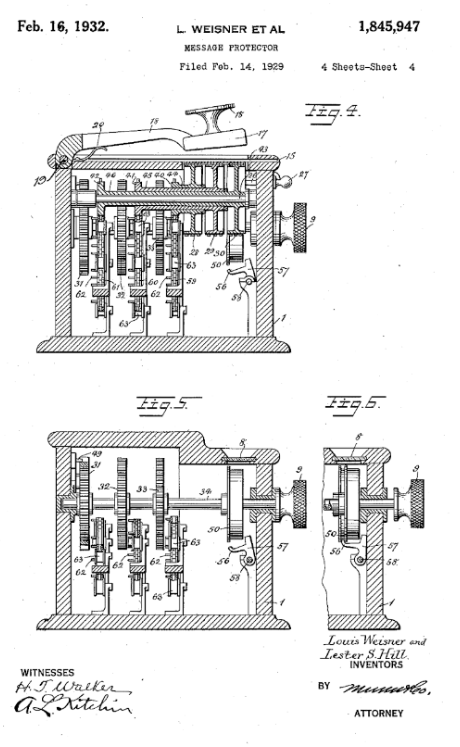
\includegraphics[width=30mm]{patent_1.png}} &
      \addheight{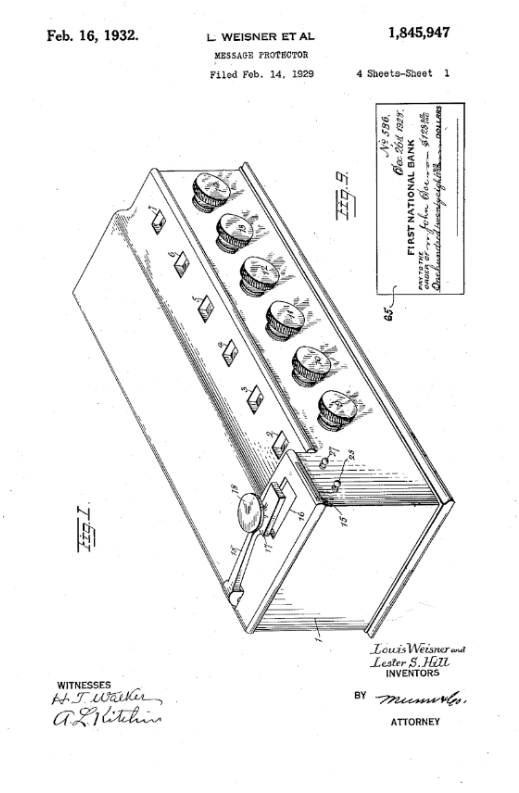
\includegraphics[width=30mm]{patent_2.png}} &
      \addheight{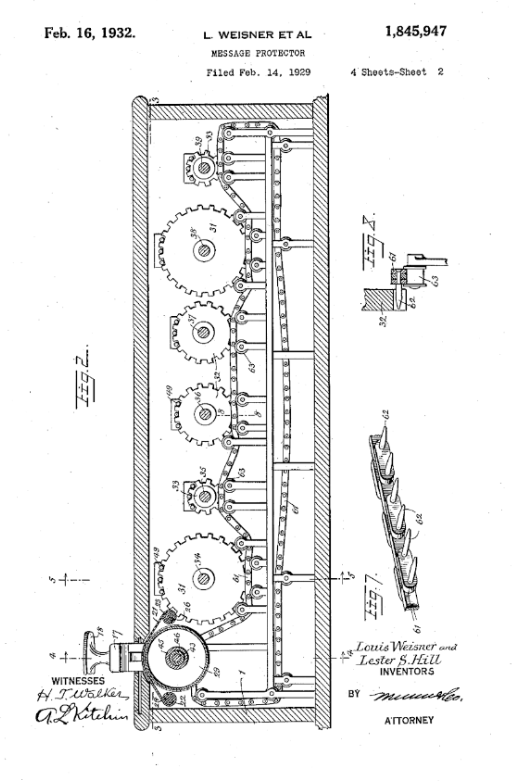
\includegraphics[width=30mm]{patent_3.png}} &
      \addheight{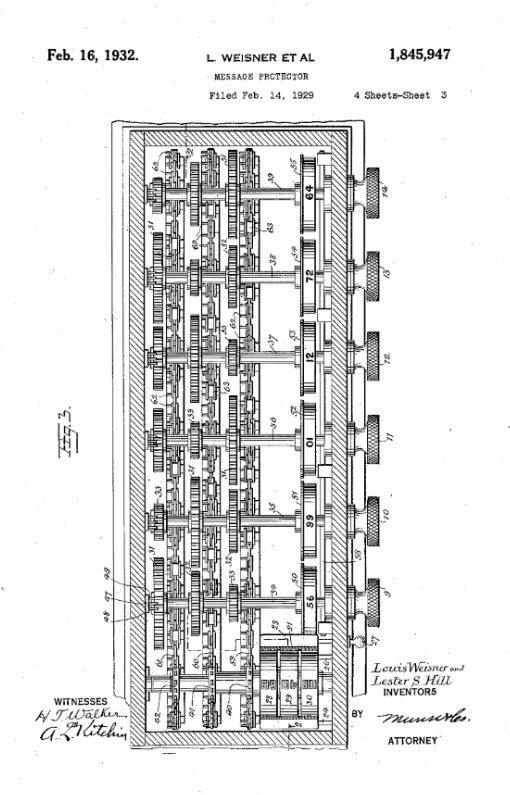
\includegraphics[width=30mm]{patent_4.png}}\\
      \hline
\end{tabular}   

\end{center}

\noindent
The significance of the Hill cipher is its implementation of advanced mathematics is one of its first. Previous ciphers mainly were based on patterns and hidden behind basic diffusion, for example, the Cesar Cipher where “both sender and receiver agree on a ‘secret shift number’ for shifting the alphabet. This number which is between 0 and 25 becomes the key of encryption.” (“Traditional Ciphers”) or the Playfair Cipher where “pairs of letters are encrypted, instead of single letters” (“Traditional Ciphers”).
\\

\section*{Linear Algebra}
\subsection*{Matrix Multiplication}
The Hill Cipher method requires knowledge of linear algebra, notably matrix multiplication, in order to be utilized. The most crucial parameter for matrix multiplication is that both matrices must adhere to the size of nxm multiplied by mxv, resulting in a matrix of size nxv, meaning that the two inner dimensions must be identical. It is impossible to do matrix multiplication if the inner dimensions do not match. For instance, the graphic below depicts a 3x3 matrix being multiplied by a 3x3 matrix, resulting in a 3x3 matrix.

\begin{center}
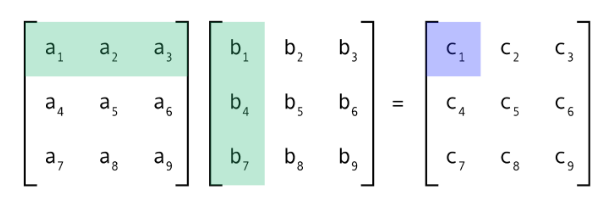
\includegraphics[width=100mm]{mmul.png}
\\
 This diagram indicates which rows and columns should be multiplied/added, as well as where the resulting answer should be placed. 
\end{center}
\subsection*{Determinate}
After multiplying the matrices, the next step is matrix inversion. To obtain the inverse of a matrix, add the identity matrix to the right-hand side of the matrix, run it through reduced row echelon form (RREF), and then multiply the inverse by the matrix discovered in the previous step (note: the inside dimensions should match so if they do not match, something is incorrect). The determinant of the matrix can also be used to determine if the inverse exists; if the determinant equals 0, then the inverse does not exist.
\begin{center}
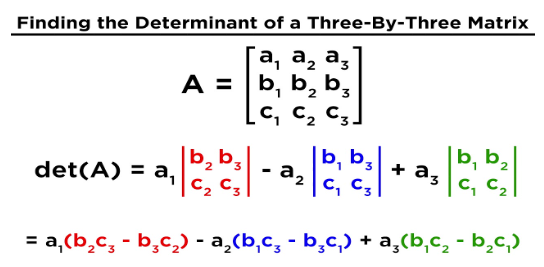
\includegraphics[width=100mm]{det.png}
\\
    This figure shows the steps to find the determinant of a 3x3 matrix.
\end{center}

The determinant is also used to determine whether the chosen key matrix is legitimate or invalid. If the determinant equals zero, the matrix is incorrect and a different key matrix must be used to decode the data.


\section*{Using a Hill Cipher}
\subsection*{Encryption}

Before we can learn how to decipher a hill cipher we must first encrypt some data using the hill cipher method

First, we will create a key we want to use and change it into a matrix using its numerical value starting at 0.
\begin
\blindtext Example: DCDF
\end{center}

\[DCDF \Rightarrow 
\begin{bmatrix}
   D& D\\
    C& F\\
  \end{bmatrix} \Rightarrow
  \begin{bmatrix}
   3& 3\\
    2& 5\\
  \end{bmatrix}\]

Then, two 2x1 matrices can be created to represent the values of the text to be encrypted. We create 2x1 matrices because we will utilize matrix multiplication with our key in the future, and we want to keep the data in 2x1 matrices.  

\[ROSE \Rightarrow 
\begin{bmatrix}
   R\\
   O\\
  \end{bmatrix} 
  \begin{bmatrix}
    S\\
    E\\
  \end{bmatrix} \Rightarrow
  \begin{bmatrix}
   17\\
   14\\
  \end{bmatrix}
  \begin{bmatrix}
   18\\
   4\\
  \end{bmatrix}
\]

  \\
\[\begin{bmatrix}
   D& D\\
    C& F\\
  \end{bmatrix} * \begin{bmatrix}
   R\\
   O\\
  \end{bmatrix} \Rightarrow
    \begin{bmatrix}
    3& 3\\
    2& 5\\
  \end{bmatrix}
   \begin{bmatrix}
   17\\
   14\\
  \end{bmatrix} = \begin{bmatrix}
   93\\
   104\\
  \end{bmatrix} \% 26 = \begin{bmatrix}
   15\\
   0\\
  \end{bmatrix} \Rightarrow
  \begin{bmatrix}
   P\\
   A\\
  \end{bmatrix}
  \]
  
   \\
\[\begin{bmatrix}
   D& D\\
    C& F\\
  \end{bmatrix} * \begin{bmatrix}
   S\\
   E\\
  \end{bmatrix} \Rightarrow
    \begin{bmatrix}
   3& 3\\
    2& 5\\
  \end{bmatrix}
   \begin{bmatrix}
   18\\
    4\\
  \end{bmatrix} = \begin{bmatrix}
   66\\
   56\\
  \end{bmatrix} \% 26 = \begin{bmatrix}
   14\\
   4\\
\end{bmatrix}\Rightarrow
  \begin{bmatrix}
   O\\
   E\\
  \end{bmatrix}
  \]

  \begin{center}
  \blindtext 
   Encrypted Data = PAOE
\end{center}
 
  
\subsection*{Decryption}
Below is the algorithm for decrypting the Hill Cipher. The given key example is solvable since it is invertible modulo 26. The Extended Euclidean Algorithm can be used to determine whether a key is invertible, but the vast majority of keys are not invertible modulo 26. The example below omits the Extended Euclidean Algorithm's proofs.
  \[K^{\!-1} \% 26=
  \begin{bmatrix}
  D& D\\
    C& F\\
  \end{bmatrix}^{\!-1}\%26=
  \begin{bmatrix}
   3& 3\\
    2& 5\\
  \end{bmatrix}^{\!-1}\%26\]
 \begin{center}
     Extended Euclidean Algorithm
 \end{center}
  \[
    ((3*5)-(3*2))^{\!-1}
    \begin{bmatrix}
   5& -3\\
    2& 3\\
  \end{bmatrix}=
  3 \begin{bmatrix}
   5& 23\\
    24& 3\\
  \end{bmatrix} =
  \begin{bmatrix}
   15& 69\\
    72& 9\\
  \end{bmatrix} \% 26 =
  \begin{bmatrix}
   15& 17\\
    20 & 9\\
  \end{bmatrix}\]
\\
  Now that we have the inverse of the key matrix, we can utilize this result to decrypt our encrypted data. With our 2x1 encrypted matrices, we will do matrix multiplication to accomplish this.
\\ 
\[
    \begin{bmatrix}
   15& 17\\
    20 & 9\\
  \end{bmatrix}
  \begin{bmatrix}
   15\\
    0\\
  \end{bmatrix} =
  \begin{bmatrix}
   225\\
    300\\
  \end{bmatrix} \% 26 = 
   \begin{bmatrix}
   17\\
    14\\
  \end{bmatrix} \rightarrow
   \begin{bmatrix}
   R\\
    O\\
  \end{bmatrix}
  \]
  
\[
    \begin{bmatrix}
   15& 17\\
    20 & 9\\
  \end{bmatrix}
  \begin{bmatrix}
   14\\
    4\\
  \end{bmatrix} =
  \begin{bmatrix}
   278\\
    316\\
  \end{bmatrix} \% 26 = 
   \begin{bmatrix}
   18\\
    4\\
  \end{bmatrix} \rightarrow
   \begin{bmatrix}
   S\\
    E\\
  \end{bmatrix}
  \]


  \begin{center}
      Decrypted Text = ROSE
  \end{center}


\section*{Modern Hill Cipher Decryption}


\subsection*{Kirchhoff principle}
Due to its poor security, the Hill Cipher is no longer utilized in modern encryption systems. In accordance with many of Kirchhoff's principles, which stipulate that the security of a cipher cannot depend on the security of the key, this is a blatant violation. The hill cipher fails the first two of Kirchhoff's six principles because it can be easily broken through brute force or frequency analysis. If the key falls into the hands of someone who knows how to use a hill cipher, the cipher can also be broken.
\begin{center}
    

1. The system must be practical, if not mathematically, indecipherable;
\\
2. It should not require secrecy, and it should not be a problem if it falls into enemy hands;\end{center}
\begin{center}
(Crypto-it. Kerckhoffs's Principle | Cryptography. (n.d.). Retrieved December 1, 2022, from http://www.crypto-it.net/eng/theory/kerckhoffs.html)
\end{center}


\subsection*{Brute Force}
\par For deciphering the Hill Cipher, brute force is an option. The cipher's key can be determined either randomly or with some degree of precision. For the hill cipher, we can make more accurate estimates if we select any key that has an inverse; with a $nxn$ matrix and $26^n$ possible permutations of matrices, there will be a huge number of keys that lack a direct inverse. Once we begin inserting random values into our matrix, we will need to cross-reference our outputs with a four-letter dictionary to determine if any outputs match the words. This method of deciphering the cipher has a high probability of yielding the incorrect answer, as the cipher could be deciphered in numerous but statistically unlikely ways. Due to the small number of guesses, especially using a 2x2 matrix, $26^4$ (456976), any current computer would be able to answer this problem in a matter of seconds. This strategy would result in us obtaining the correct answer in the most time. This method does not necessarily solve the cipher; it simply yields the correct answer after a lengthy period of time compared to using different approaches to decryption.
\par
 This code demonstrates how to brute-force the Hill Cipher's key. While not elegant, it illustrates how $26^4$ computations can be used to find all of the inverses for the data set. Putting this list back into the decryption algorithm will yield a huge number of possible ciphertext solutions. Few of these will provide a plausible answer, while the majority will be illogical. This method additionally has a skip for singular inverses that would not provide a proper key, thus reducing the data set.

\begin{center}
 This code can be thought of as performing the following stages without a dictionary lookup. 
\end{center}

  \[K^{\!-1} \% 26=
  \begin{bmatrix}
 i& j\\
    k& l\\
  \end{bmatrix}^{\!-1}\%26\]
 
\begin{mintedbox}{python}
from numpy import *
import numpy as np
for i, in range(1, 26):
    for j in range(1, 26):
        for k in range(1, 26):
            for l in range(1, 26):
                try:
                    K = np.array([[i, j],
                                [k, l]])
                except np.linalg.LinAlgError:
                    print('Singular Matrix')

\end{mintedbox}
\\

\subsection*{Frequency Analysis
}
Similarly, we find letters that occur more frequently in the ciphers. It is likely that there is a correlation and using these letters in pairs, we can begin to formulate guesses at the keys. For example, matching the most frequent letter pair in a cipher of SW to ET may lead to successful deciphering. While this technique does involve guessing the key and is similar to brute force, in simple ciphers it sufficiently reduces the number of guesses needed. So substantially that most ciphers become decipherable by hand. With the aid of a computer, even one as simple as a graphing calculator, deciphering becomes trivial.

  
\section*{Conclusion}
We initially felt that it was possible to use the Hill cipher to develop a more powerful encrypted cipher, but we quickly discovered that this is not the case, as the Hill Cipher is extremely simple to solve in the modern era. Using this information, we were able to build and comprehend several methods for deciphering ciphers and what makes a good cipher good. The concepts of Kirchhoff greatly improved our understanding of what a successful cipher requires. To improve data encryption in the future, the focus of the research would move to discovering ciphers that adhere to Kirchhoff's principles. Even if we didn't need to find a way to implement the Hill cipher in modern applications, we still learnt a great deal about what makes linear algebra an excellent technique to encrypt various data sources if they can follow Kirchhoff's principle.

  
\end{document}